\documentclass{standalone}
\usepackage{ tikz }
\usetikzlibrary{shapes}
\usetikzlibrary{plotmarks}
\usepackage{amsmath}
\usepackage{ xparse }
\usepackage{../../../macros}

\begin{document}
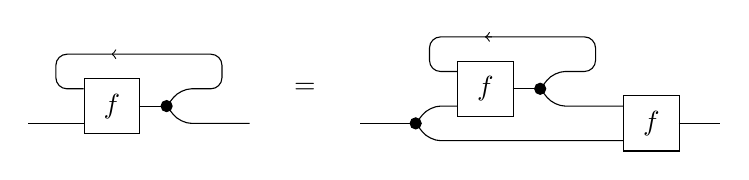
\begin{tikzpicture}[yscale=-1,x=1em,y=1.25em]
        
    \node at (0,-2.5) {};

    \draw (-1,0) -- (1,0);
    \node[draw, minimum height = 2em, minimum width = 2em, anchor = west] at (1,-0.5){$f$};
    \draw (3,-0.5) -- (4,-0.5);
    \filldraw (4,-0.5) circle (2pt);
    \draw [rounded corners, ->] (4,-0.5) -- (4.5,-1) -- (6,-1) -- (6, -2) -- (2, -2);
    \draw [rounded corners] (2,-2) -- (0,-2) -- (0,-1) -- (1,-1);
    \draw [rounded corners] (4,-0.5) -- (4.5, 0) -- (7,0);

    \node at (9,-1) {$=$};

    \draw (11, 0) -- (13,0);
    \filldraw (13,0) circle (2pt);
    \draw [rounded corners] (13,0) -- (13.5,-0.5) -- (14.5, -0.5);
    \draw [rounded corners] (13,0) -- (13.5,0.5) -- (20.5,0.5);
    \node[draw, minimum height = 2em, minimum width = 2em, anchor = west] at (14.5,-1){$f$};
    \draw (16.5,-1) -- (17.5,-1);
    \filldraw (17.5,-1) circle (2pt);
    \draw [->, rounded corners] (17.5,-1) -- (18,-1.5) -- (19.5,-1.5) -- (19.5, -2.5) -- (15.5, -2.5);
    \draw [rounded corners] (15.75, -2.5) -- (13.5,-2.5) -- (13.5, -1.5) -- (14.5,-1.5);
    \draw [rounded corners] (17.5,-1) -- (18,-0.5) -- (20.5,-0.5);
    \node[draw, minimum height = 2em, minimum width = 2em, anchor = west] at (20.5,0){$f$};
    \draw (22.5,0) -- (24,0);

\end{tikzpicture}
\end{document}